% IEEE Transactions / journal article. "journal" is what separates this from the
% conference template: a running header (\markboth), a drop-cap first word, a biography
% for every author at the end, and the page footer for the published volume.
% Add "draftcls,onecolumn" while writing if you want a roomy, single-column draft.
\documentclass[journal]{IEEEtran}
\usepackage{amsmath,amssymb}
\usepackage{graphicx}
\usepackage{booktabs}
\usepackage{tikz}
\usepackage{cite}

% IEEE journals ask for "et al." in italics in the header, hence \MakeLowercase{\textit{et al.}}.
% Replace the journal name, volume and date with what the editorial office gives you.
\markboth{IEEE Transactions on Example Systems, Vol.~XX, No.~X, Month 2026}%
{Author \MakeLowercase{\textit{et al.}}: Title of Your Journal Article}

\begin{document}

\title{Title of Your Journal Article: Keep It Specific and Short}

% \IEEEmembership goes after the name; leave it out if an author is not a member.
\author{First~Author,~\IEEEmembership{Member,~IEEE,}
        and~Second~Author,~\IEEEmembership{Senior Member,~IEEE}%
\thanks{Manuscript received Month DD, 2026; revised Month DD, 2026. This work was
supported by Funding Body under Grant 000000. (Corresponding author: First Author.)}%
\thanks{First Author is with the Department of Electrical Engineering,
Example University, City, Country (e-mail: first.author@example.edu).}%
\thanks{Second Author is with Example Research Lab, City, Country.}}

\maketitle

\begin{abstract}
Summarise the problem, your approach and the main result in a single paragraph of 150 to
250 words. Do not cite references, use displayed equations or refer to figures here:
the abstract is indexed on its own.
\end{abstract}

\begin{IEEEkeywords}
Keyword one, keyword two, keyword three (alphabetical order, from the IEEE Taxonomy).
\end{IEEEkeywords}

\section{Introduction}
\IEEEPARstart{S}{tate} the problem, why it matters and what is missing in earlier work in
the first paragraph; \verb|\IEEEPARstart| sets the large first letter that IEEE journals
use. Then list your contributions: we (i) propose a method, (ii) prove a bound on its
error, and (iii) evaluate it on three data sets. Cite as in~\cite{shannon48,knuth84}.

\section{Method}\label{sec:method}
Describe the system or algorithm. Equations are numbered automatically:
\begin{equation}
  y[n] = \sum_{k=0}^{N-1} h[k]\, x[n-k] .
  \label{eq:fir}
\end{equation}
Refer to them as~\eqref{eq:fir}, to sections as Section~\ref{sec:results}, and to the
proof in Appendix~\ref{app:proof}.

\subsection{Assumptions}
Subsections are numbered with capital letters and appear in italics in IEEE journals.

\section{Results}\label{sec:results}
Table~\ref{tab:results} shows how results are typeset: IEEE puts table captions above
the table (in small capitals) and figure captions below the figure.

\begin{table}[!t]
  \caption{Comparison of the baseline and the proposed method}
  \label{tab:results}
  \centering
  \begin{tabular}{lcc}
    \toprule
    Method & Error (\%) & Time (ms) \\
    \midrule
    Baseline & 12.4 & 38 \\
    Proposed & 8.1 & 41 \\
    \bottomrule
  \end{tabular}
\end{table}

\begin{figure}[!t]
  \centering
  % A small figure drawn in TikZ; replace with \includegraphics[width=\columnwidth]{fig.pdf}.
  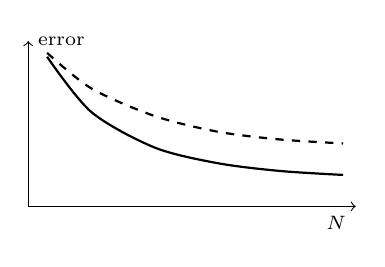
\begin{tikzpicture}[x=0.8cm,y=0.5cm]
    \draw[->] (0,0) -- (5.2,0) node[below left] {\scriptsize $N$};
    \draw[->] (0,0) -- (0,4.2) node[right] {\scriptsize error};
    \draw[thick] plot[smooth] coordinates {(0.3,3.8) (1,2.4) (2,1.5) (3,1.1) (4,0.9) (5,0.8)};
    \draw[thick,dashed] plot[smooth] coordinates {(0.3,3.9) (1,3.0) (2,2.3) (3,1.9) (4,1.7) (5,1.6)};
  \end{tikzpicture}
  \caption{A figure that fits one column (solid: proposed, dashed: baseline). Use
  \texttt{figure*} for both columns.}
  \label{fig:error}
\end{figure}

\section{Conclusion}
Repeat the contribution in one sentence, then name the most useful future work.

% Appendices: one gets no letter, several are numbered A, B, ... by \appendices.
\appendices
\section{Proof of the Error Bound}\label{app:proof}
Put long derivations here so the main text stays readable.

% The heading is unnumbered on purpose; IEEE uses "Acknowledgment" without the extra "e".
\section*{Acknowledgment}
Thank colleagues and, if not already in the first footnote, the funding bodies.

\bibliographystyle{IEEEtran}
\bibliography{refs}

% IEEE journals print a short biography of every author. The photo is 1 inch wide and
% 1.25 inches high; the box below is a placeholder, replace it with
% \includegraphics[width=1in,height=1.25in,clip,keepaspectratio]{photo.jpg}.
\begin{IEEEbiography}[{%
  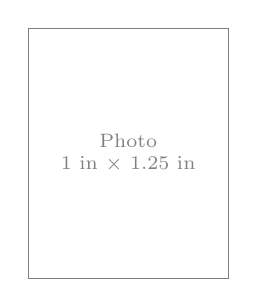
\begin{tikzpicture}
    \draw[gray] (0,0) rectangle (1in,1.25in);
    \node[gray,align=center,font=\scriptsize] at (0.5in,0.625in) {Photo\\1 in $\times$ 1.25 in};
  \end{tikzpicture}}]{First Author}
(Member, IEEE) received the B.S. and Ph.D. degrees in electrical engineering from
Example University, City, Country, in 2015 and 2020. Say where they work now and what
their research interests are, in 100 words or fewer.
\end{IEEEbiography}

% Authors without a photo (allowed for some journals) use this shorter form.
\begin{IEEEbiographynophoto}{Second Author}
(Senior Member, IEEE) is with Example Research Lab. Describe education, employment and
interests in the same style.
\end{IEEEbiographynophoto}

\end{document}
